\chapter{Cascade of Transducers}
\label{chap-cassys}

The general principle of a \textit{cascade of transducer} \index{cascade of transducer}  to apply several transducers the one 
after the other on a text to modify the text. Under Unitex, a transducer is a graph, 
compiled in fst2 format. Such a system can be used to analyze a text in different ways: 
syntactic analysis, chunking, information extraction or simply to transform a text for other purpose.

\bigskip
\noindent The prototype of the \textit{CasSys} \index{CasSys} system was created in 2002 at the LI 
(Computer science laboratory of the university of Tours) during the thesis of Nathalie Friburger (\cite{reco-np-friburger02}). 
Then, it was fully dedicated to named entity extraction. CasSys was generalized to allow any sort of work needing a cascade:
 it was improved as one goes along but not really integrated in Unitex. 
 Finally, it has been integrated to unitex by David Nott and Nathalie Friburger thanks to a Feder project launched by Denis Maurel.
A priori, the use of cassys is roughly a succession of locate patterns eventually with special options. 

\bigskip
\noindent In this chapter, we will explain how to create cascades of transducers and use CasSys.

%%%%%%%%%%%%%%%%%%%%%%%%%%%%%%%%%%%%%%%%%%%%%%%%%%%%%%%%%%%%%
\section{Applying a cascade of transducer with CasSys}
\label{section:applyCascade}

In the text menu, you can select the submenu "Apply CasSys cascade..." (\ref{fig13-01}) which opens the CasSys window.
This submenu "Apply CasSys cascade" becomes active only if you have opened a text.

\begin{figure}[!htb]
 \centering
 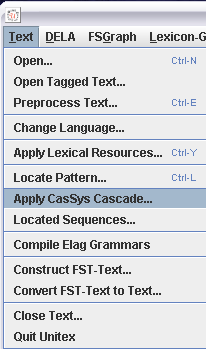
\includegraphics[width=2.8cm]{resources/img/fig13-01.png}
 \caption{Text menu of Unitex and submenu Apply CasSys Cascade}
 \label{fig:fig13-01}
\end{figure}


\subsection{Creating a list of transducer to apply}
\label{subsec:listTrans}

The list of transducers of a cascade is saved in a text file with the extent csc (ex: mycascade.csc).

\bigskip
\noindent In order to create the list of transducer, you can click on the "new" button of the cassys window. 
If you want to modify an existing cascade, you can choose the file name of the cascade, then click on the "edit" button. 
Those buttons open the "CasSys transducer configuration" window.

\subsection{Editing the list of transducers}
\label{subsec:editlistTrans}

The Cassys Transducer configuration window (\ref{fig13-03}) is defined in three parts :

\begin{figure}[!htb]
  \centering
  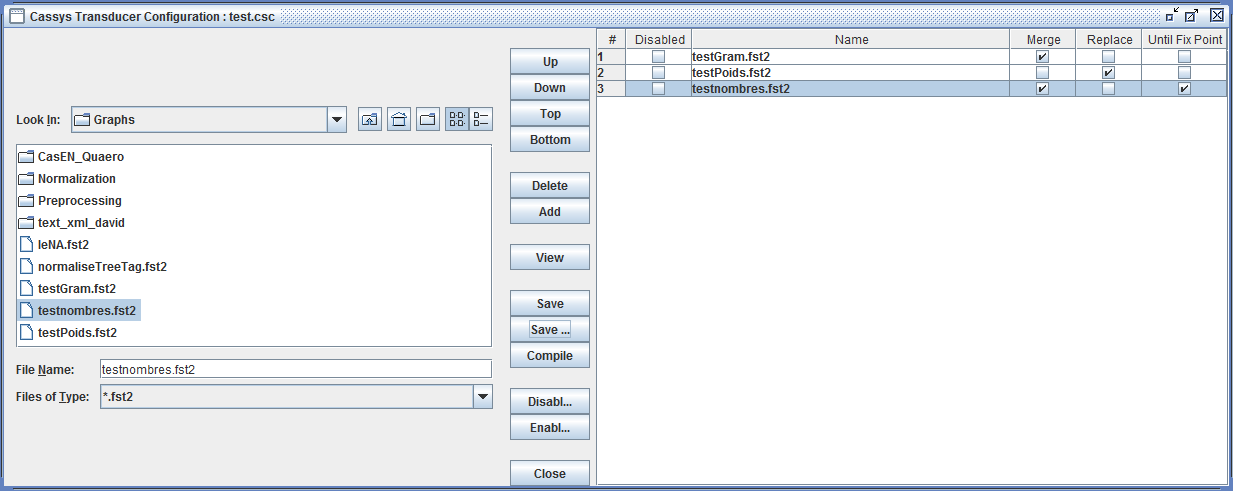
\includegraphics[width=10cm]{resources/img/fig13-03.png}
  \caption{Cassys Transducer configuration window with a list of transducer at the right}
  \label{fig:fig13-03}
\end{figure}

\begin{itemize}
	\item The left of the Cassys Transducer configuration window contains a file explorer to choose the transducers to add to the cascade. 
	The file explorer only displays the fst2 files (all the graphs you want to place in the list of transducer must be compiled in fst2 format). 
	To edit the cascade, you must choose the graphs in the file explorer and drag and drop this file from the left to the right of the windows.
	\item At the right, there is the list of transducer (empty if you create a new cascade).
	The list of transducer is ordered : the first graph of the list is applied in first, and the last at the end. The list is composed of three columns: the first contains 	the name of each graphs, the second the option merge, the third the optioin replace. You must choose between merge or replace which are the manner to take into account 	the outputs of the graphs (like in the locate pattern program). Merge indicates that the outputs of a graph will be merged to the text whereas replace will replace the 	recognized text by the outputs of the graph. For a cascade of transducer, it has no sense to not take into account outputs : this is why this option is not proposed 		here.
 	When the cassys transducer configuration window opens the list of transducer, it verifies if all the files of the list of transducer exist or not: if a file does not 	exist, it appears in red in the list (perhaps you have forgotten to compile the graph into fst2). 
	When you let the mouse a few seconds on the file name, all the path appeared. 
	\item In the middle, different buttons to do some actions. 
		\begin{itemize}
			\item The up/down/top/bottom buttons are used to modify the order of the transducers in the list (it moves the selected transducer in the list) ; 
			up and down to move the selected transducer one line above respectively below, and top and down to move the selection at the top of list or at the end.
			\item  The Delete button permits to suppress a selected transducer in the list of transducers. The Add button adds a transducer (previously selected in the explorer) in the list. The Add button do the same thing than drag and drop a transducer. 
			\item The View button opens the graph selected either in the file explorer or in the list of transducer of the window. It is useful to seek quickly a transducer to see its contain and to modify it.
			\item The Save button and Save as button permit to save the list of transducer. By default, the lists of transducers are stored in the cassys folder of the current language (e.g. English/Cassys).
			\item The Close button to close the current window.
		\end{itemize}
\end{itemize}

\subsection{Launching a cascade}
\label{subsec:launchCascade}

The CasSys window (\ref{fig13-02}) displays the contain of the cassys folder of the current language. It permits to choose 
the file containing the list of transducer to apply on the text. The files displayed are in a special file type "CaSCade configuration file" (.csc). 
When this list is chosen, you can click on the "Launch" button to apply the cascade.

\begin{figure}[!htb]
  \centering
  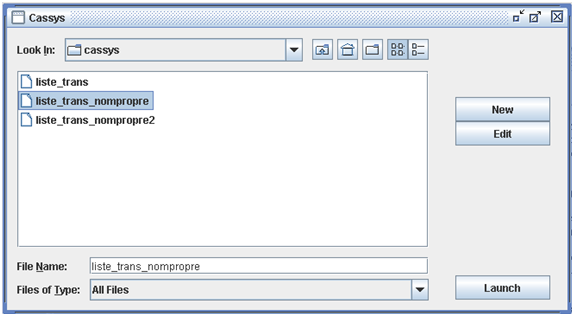
\includegraphics[width=10cm]{resources/img/fig13-02.png}
  \caption{CasSys Window to launch a cascade of transducer}
  \label{fig:fig13-02}
\end{figure}

\subsection{Viewing the results of a cascade}
\label{subsec:resultsCascade}

The result of the cascade is an index file (concord.ind) like for the locate pattern operation. This index file contains all the sequences recognized with the restriction imposed by the rules of unitex.

\bigskip
\noindent In order to display a concordance, you have to click on the build concordance button (as described in Chapter \ref{chap-advanced-grammars}) 
in the menu text / located sequences (\ref{fig13-04} presents a sample of concordance on the results of a cascade recognizing named entities).
To create the file containing all the modification of the cascade on the text, you have to click on Modify text in the Located Sequences window.
 The resulting file is a copy of the text in which transducer outputs have been taken into account.

\begin{figure}[!htb]
  \centering
  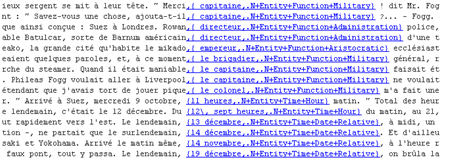
\includegraphics[width=14cm]{resources/img/fig13-04.png}
  \caption{Concordance of Cassys under Unitex}
  \label{fig:fig13-04}
\end{figure}

%%%%%%%%%%%%%%%%%%%%%%%%%%%%%%%%%%%%%%%%%%%%%%%%%%%%%%%
\section{Details on Cassys}

In this section , we present details concerning the behaviour of Cassys.

\subsection{Type of graphs used}

Cassys used the compiled version of the graphs (the fst2 files).
Cassys can handle the local grammars (section 6.1) (syntactic graphs) presented in Chapter \ref{chap-advanced-grammars}. Those grammars can use subgraphs, 
morphological filters and mode,and allow to refer to information in dictionaries. 
The grammars used in the cascade must follow the constraints on unitex grammars.

\subsection{The unitex rules used for the cascade}

In the cascade, each succeeding graphs are applied with the following unitex rules:
\begin{itemize}
	\item Insertion to the left of the matched patterns : in the merge mode, the ouput is inserted to the left of the recognized sequence.
	\item	Priority of the leftmost match : during the application of a local grammar, overlapping occurrences are all indexed. 
	During the construction of a concordance, all these overlapping occurrences are presentend but cassys modifies the text with each 
	graph of the cascade : so it is needed to choose among these occurrences the one that will be taken into account. The priority rule 
	is the leftmost sequence.
	\item Priority of the longest match : for cassys, during the application of a graph, it is the longest sequence 
	that will be keeped.
	\item	Search limitation to a certain number of occurrences: For Cassys, this search is not limited; we index all utterances in the text.
\end{itemize}

\subsection{The special way to mark up patterns with cassys}

The output of the transducers can be used to insert in texts special information, particularly to mark up the patterns recognized : it is 
possible to use all the mark you want, like ( ), [], "", or xml like (<xxx> </xxx>) etc., but Cassys proposes a special way to 
mark up patterns that offers some advantage and that we present here.  

\bigskip
\noindent Unitex splits texts in different sort of tokens like the sentence delimiter {S}; the stop marker {STOP}, contiguous 
sequences of letters, lexical tags {aujourd'hui,.ADV}, etc. The lexical tag is used by cassys in a special way. The lexical tag (between curly brackets) is normally used to avoid ambiguities (see explanation in section \ref{tokenization} and in section\ref{section-displaying-sentence-automata}). 
For example, in a text, if you have the token \{curly brackets,.N\}, neither "curly" nor "brackets" will be recognized but the whole sequence 
"curly brackets". A lexical tag can contains complex lexical information like N+Pers+Hum:fs.
In a graph, you can search lexical token by the lexical information they contain: for example, you can write <N> to search 
a noun, <Pers+Hum> for a human person or <pers-Hum> for a non human person. Those lexical masks are explained in the Chapter Searching with Regular Expressions in the section \ref{section-special-symbols}.
 
\bigskip
\noindent In Cassys, we use the lexical tag in a special way. A cascade of transducer is interesting to search the island of certainty first. It is necessary for such a system to prevent the already recognized patterns to be ambiguous with following sequences. To do that, you can tag patterns of your graphs surrounding them by \emph{\{} and \emph{,.tag1+tag2+tagn\}} in the outputs of the graph.

\bigskip
\noindent To explain this behavior, here is a very simple example. The text on which we work is :
\emph{bac a b c cc a b b ba ab a b bca a b c abaabc}.

\bigskip
\noindent The graph grfAB (\ref{fig13-05}) recognizes the sequence ab in the text and tag this sequence as lexical tag {a b,.AB}. This graph is merged with the text and adds its outputs \{ and ,.AB\} to the text. 

\begin{figure}[!htb]
  \centering
  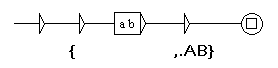
\includegraphics[width=9cm]{resources/img/fig13-05.png}
  \caption{the graph grfAB}
  \label{fig:fig13-05}
\end{figure}

\bigskip
\noindent The resulting text is : \emph{bac \{a b,.AB\} c cc \{a b,.AB\} b ba ab \{a b,.AB\} bca \{a b,.AB\} c abaabc}.

\bigskip
\noindent Now the pattern ab is tagged AB. A part (a or b alone) of this pattern cannot be recognized because of the tagging of a b. 

\bigskip
\noindent After that graph, the cascade applies another graph named tagAB (\ref{fig13-06}) contains the lexical masks <AB>. It recognizes all the sequence lexically tagged by the previous graph.

\begin{figure}[!htb]
  \centering
  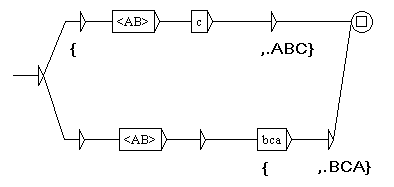
\includegraphics[width=10cm]{resources/img/fig13-06.png}
  \caption{the graph tagAB}
  \label{fig:fig13-06}
\end{figure}

\bigskip
\noindent The resulting text is : \emph{bac \{\{a b,.AB\} c,.ABC\} cc \{a b,.AB\} b ba ab \{a b,.AB\} \{bca,.BCA\} \{\{a b,.AB\} c,.ABC\} abaabc}.

% \#M
% 2.0.0 6.0.0 \{\\\{a b\\,\\.AB\\\} c,.ABC\}
% 10.0.0 12.0.0 \{a b,.AB\}
% 20.0.0 24.2.0 \{a b,.AB\} \{bca,.BCA\}
% 26.0.0 30.0.0 \{\\\{a b\\,\\.AB\\\} c,.ABC\}

\bigskip
\noindent The concordance displayed by unitex should be like in (\ref{fig13-07}). For programming reasons (ambiguities between characters in the curly brackets of the lexical tags), we are constrained to place backslashes \\ before all ambiguous characters ; that's why those symbols are protected with \\ in the concordance to avoid problems in unitex. 

\begin{figure}[!htb]
  \centering
  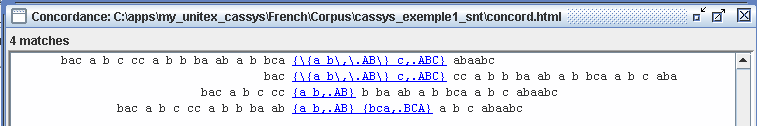
\includegraphics[width=12cm]{resources/img/fig13-07.png}
  \caption{the concordance resulting of this cascade}
  \label{fig:fig13-07}
\end{figure}

\bigskip
\noindent This examples show that the writing of graphs using the lexical tags placed by preceeding graphs is very simple. The tags can be overlapped each other.

\subsection{Interest of a cascade of transducer}

Unitex grammars are known as Context free grammars and contain the notion of transduction derived from the field 
of finite state automata. A grammar with transduction (a transducer) is enabled to produce some ouput. 
Cassys is dedicated to apply transducers in cascade.

\bigskip
\noindent The transducers are interesting because they permits to associate a recognized sequence with informations in outputs of the graphs. 

\bigskip
\noindent This outputs can :
\begin{itemize}
	\item	Be merged with the recognized sequence found in the text and appear in the resulting concordance or modified text. 
	\item	Replaced the recognized sequence to modify the text. 
\end{itemize}

\bigskip
\noindent Those two operations transform the text, add informations in the text for different purpose or modify it. It can be used to do syntactic analysis, 
chunking, information extraction, etc. 

\bigskip
\noindent The advantage of a cascade is mainly that it's a good way to manage priority between patterns that you want find in a text. If you know two ambiguous pattern, you can applied the less ambiguous pattern first.

\subsection{The longest pattern}

The heuristic of the longest pattern matching is applied for each transducer of the cascade. When a graph is applied to a text, several path can be recognized
by the graph. 

\bigskip
\noindent If the graph arrives to its final state by several paths then it is the path that recognizes the longest pattern that is chosen. The longest is
the pattern, less ambiguous it is.
If the transducer don't arrive on the final state then the recognizing restarts on the nex word of the text.

\bigskip
\noindent The longest pattern matching heuristic is interestinf but if several paths of the same size are recognized there is still a problem; one of the paths will be chosen without having the control on this choice: the worst can be chosen.
That's why a solution can be to create a cascade of transducer to give the priority of the best paths.

\bigskip
\noindent If a graph contains two paths that are ambiguous each with the other, one can creat two graphs containing each one of the paths. 
The first graph will contain the safest path, the second the less safe.

\bigskip
\noindent Cassys keeps all the text created by each graph of the cascade. It is useful to test, debug or check the different results of the cascade. It is possible 
to correct the errors on the order of the graphs or to find the errors in the writing of the graphs. To help, a good idea is to place the name of the transducer recognizing a pattern in the outputs of the graphs: thanks to that, you can see in the final results by what graph is recognized a pattern. 

\subsection{Files resulting of cassys}

If you apply a cascade on the text named example.txt.
Two folders are created: example\_snt and example\_csc.
The files produced in example\_csc are mainly the results of each graphs in files numbered with the order number of the graph that produces the file (if the third graph
finds a pattern, cassys produces a texte named example\_3.snt).
